\graphicspath{{content/title/figures/}}

\begin{titlepage}

\begin{center}

\begin{tabular}{ p{2cm} p{2cm} p{8cm} p{2cm}}
\multirow{3}{*}{
\includegraphics[width=1.45cm]{logo_upt}} &
\multirow{3}{*}{
\includegraphics[width=1.55cm]{logo_college}} &
\small{Universitatea ``Politehinca'' Timi\c{s}oara} &
\multirow{3}{*}{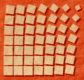
\includegraphics[width=1.55cm]{logo_departament}} \\
& & \small{Facultatea de Automatic\u{a} \c{s}i Calculatoare} & \\
& & \small{Departamentul Calculatoare} & \\
& & \tiny{2, Vasile P\u{a}rvan Bv., 300223 � Timi\c{s}oara, Romania}\\
& & \tiny{Tel: +40 256 403261,  Fax: +40 256 403214}\\
& & \tiny{Web: http://www.cs.upt.ro}\\
\end{tabular}

\vspace{5cm}

\Huge

Corectarea automat'a a condi'tiilor de curs'a 'in programe Java concurente
folosind privatizarea de date.

\large

\vspace{1.6cm}

\sc{Rezumat Lucrare de Licen\c{t}a}

\vspace{4cm}

\begin{minipage}{0.55\textwidth}
\begin{flushleft} \large
\emph{Coordonatori stiin'tifici:} \\
{\sc Danny Dig} \\
{\sc Marius Minea}
\end{flushleft}
\end{minipage}
\begin{minipage}{0.4\textwidth}
\begin{flushright} \large
\emph{Autor:}\\
\sc{Lor\'{a}nd Szak\'{a}cs}
\end{flushright}
\end{minipage}


\vfill

\normalsize

Timi\c{s}oara \\
2012

\end{center}

\end{titlepage}